\section{Sơ Đồ Kiến Trúc Tổng Quan Của Sản Phẩm}

\subsection{Giới Thiệu}

Chương này trình bày sơ đồ kiến trúc tổng quan của sản phẩm và giải thích chi tiết từng thành phần của kiến trúc đó.

\subsection{Sơ Đồ Kiến Trúc Tổng Quan}

\begin{figure}[H]
\centering
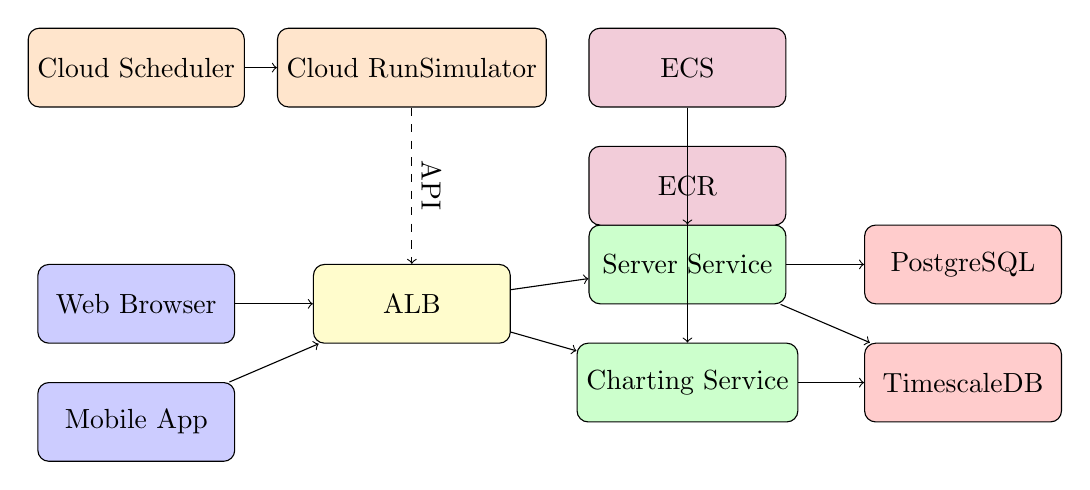
\begin{tikzpicture}[
    node distance=1.5cm and 2cm,
    box/.style={rectangle, draw, minimum width=2.5cm, minimum height=1cm, text centered, rounded corners},
    client/.style={box, fill=blue!20},
    gateway/.style={box, fill=yellow!20},
    app/.style={box, fill=green!20},
    data/.style={box, fill=red!20},
    cloud/.style={box, fill=purple!20},
    gcp/.style={box, fill=orange!20}
]
    % Client Layer
    \node[client] (web) {Web Browser};
    \node[client, below of=web] (mobile) {Mobile App};
    
    % API Gateway
    \node[gateway, right of=web, xshift=2cm] (gateway) {ALB};
    
    % Application Layer (AWS)
    \node[app, right of=gateway, xshift=2cm, yshift=0.5cm] (server) {Server Service};
    \node[app, below of=server] (charting) {Charting Service};
    
    % Data Layer (AWS)
    \node[data, right of=server, xshift=2cm] (postgres) {PostgreSQL};
    \node[data, below of=postgres] (timescale) {TimescaleDB};
    
    % Google Cloud - Simulator
    \node[gcp, above of=web, yshift=1.5cm] (scheduler) {Cloud Scheduler};
    \node[gcp, right of=scheduler, xshift=2cm] (cloudrun) {Cloud Run\\Simulator};
    
    % Cloud Services (AWS)
    \node[cloud, above of=server, yshift=1cm] (ecs) {ECS};
    \node[cloud, above of=charting, yshift=1cm] (ecr) {ECR};
    
    % Connections
    \draw[->] (web) -- (gateway);
    \draw[->] (mobile) -- (gateway);
    \draw[->] (gateway) -- (server);
    \draw[->] (gateway) -- (charting);
    \draw[->] (server) -- (postgres);
    \draw[->] (server) -- (timescale);
    \draw[->] (charting) -- (timescale);
    \draw[->] (scheduler) -- (cloudrun);
    \draw[->, dashed] (cloudrun) -- node[above, sloped] {API} (gateway);
    \draw[->] (ecs) -- (server);
    \draw[->] (ecs) -- (charting);
\end{tikzpicture}
\caption{Sơ đồ kiến trúc tổng quan của sản phẩm}
\label{fig:kien-truc-tong-quan}
\end{figure}

% Lưu ý: Nếu muốn sử dụng mermaid.js, có thể:
% 1. Export mermaid diagram sang PNG/SVG từ https://mermaid.live/
% 2. Sử dụng \includegraphics để chèn hình ảnh
% 3. Hoặc sử dụng package mermaid trên Overleaf (nếu được hỗ trợ)

\subsection{Giải Thích Chi Tiết Các Thành Phần}

\subsubsection{Lớp Client (Client Layer)}

Lớp client bao gồm các ứng dụng mà người dùng cuối sử dụng để tương tác với hệ thống:

\textbf{Web Browser:}
\begin{itemize}
    \item Trình duyệt web (Chrome, Firefox, Safari, Edge) để truy cập Portal
    \item Portal là Single Page Application (SPA) được xây dựng bằng Vue.js
    \item Giao tiếp với backend thông qua RESTful API
    \item Hỗ trợ responsive design để sử dụng trên nhiều kích thước màn hình
    \item Hỗ trợ đa ngôn ngữ (i18n) với English, Spanish, và Vietnamese
\end{itemize}

\textbf{Mobile App (Tương lai):}
\begin{itemize}
    \item Hiện tại chưa có mobile app, nhưng kiến trúc API cho phép dễ dàng phát triển mobile apps trong tương lai
    \item API được thiết kế để hỗ trợ cả web và mobile clients
\end{itemize}

\subsubsection{Application Load Balancer (ALB)}

AWS Application Load Balancer đóng vai trò là entry point chính cho tất cả HTTP/HTTPS traffic:

\textbf{Chức năng:}
\begin{itemize}
    \item Nhận tất cả incoming HTTP/HTTPS requests từ internet
    \item Phân phối traffic đến các Server service instances trong ECS cluster
    \item Thực hiện health checks để đảm bảo chỉ route traffic đến healthy targets
    \item SSL/TLS termination để xử lý HTTPS connections
    \item Path-based routing (có thể mở rộng trong tương lai)
\end{itemize}

\textbf{Lợi ích:}
\begin{itemize}
    \item High availability: Đảm bảo service luôn available ngay cả khi một số tasks fail
    \item Auto-scaling support: Tự động route traffic đến new tasks khi scale up
    \item Security: Có thể tích hợp với AWS WAF để bảo vệ khỏi attacks
    \item Monitoring: Tích hợp với CloudWatch để monitor traffic và performance
\end{itemize}

\subsubsection{Lớp Ứng Dụng (Application Layer)}

Lớp ứng dụng bao gồm các microservices chạy trên ECS Fargate:

\textbf{Server Service (Go + Vue.js):} Đây là service chính của hệ thống, chứa cả backend API và frontend Portal trong một Docker container duy nhất. Kiến trúc này được gọi là "monolithic frontend" pattern, nơi backend server serve cả API và static files cho frontend. Điều này đơn giản hóa deployment vì chỉ cần deploy một service thay vì hai services riêng biệt.

\begin{itemize}
    \item \textbf{Backend API}: RESTful API được phát triển bằng Go (Golang) sử dụng framework Goa. Goa là một framework đặc biệt cho phép design-first API development, nơi API được định nghĩa bằng DSL (Domain Specific Language), sau đó code được generate tự động. Điều này đảm bảo consistency giữa API specification và implementation. API được thiết kế theo RESTful principles với các endpoints như \texttt{GET /projects}, \texttt{POST /projects}, \texttt{GET /stations}, \texttt{POST /ingestion}, v.v. Mỗi endpoint có validation, error handling, và logging được implement đầy đủ.
    
    \item \textbf{Chức năng chính của Backend API}:
        \begin{itemize}
            \item \textbf{Quản lý stations, sensors, và projects}: API cung cấp đầy đủ CRUD operations cho các entities này. Mỗi project có thể chứa nhiều stations, và mỗi station có thể có nhiều sensors. API hỗ trợ nested queries để lấy stations của một project hoặc sensors của một station.
            
            \item \textbf{Xử lý data ingestion từ IoT devices}: Endpoint \texttt{POST /ingestion} nhận data từ IoT devices. Data được validate, parse, và lưu vào database. Metadata (station, sensor info) được lưu vào PostgreSQL, trong khi time-series data (readings) được lưu vào TimescaleDB. Ingestion endpoint được tối ưu hóa để xử lý high throughput với batch processing.
            
            \item \textbf{Authentication và authorization}: API sử dụng session-based authentication với encrypted session cookies. Mỗi request được validate để đảm bảo user có quyền truy cập resource. Authorization được implement ở nhiều levels: project-level (user có thể access project hay không), station-level (user có thể access station hay không), và data-level (user có thể query data hay không).
            
            \item \textbf{CRUD operations cho tất cả entities}: API cung cấp đầy đủ Create, Read, Update, Delete operations cho users, projects, stations, sensors, và data. Mỗi operation có validation và business logic riêng. Ví dụ, khi delete một station, hệ thống cần xóa cả data liên quan trong TimescaleDB.
            
            \item \textbf{Geographic queries với PostGIS}: API hỗ trợ spatial queries để tìm stations trong một khu vực địa lý cụ thể. Ví dụ, có thể query tất cả stations trong bán kính 10km từ một điểm. PostGIS cung cấp các functions như \texttt{ST\_Distance}, \texttt{ST\_Within}, \texttt{ST\_Buffer} để thực hiện các spatial operations.
        \end{itemize}
    
    \item \textbf{Frontend Portal}: Vue.js SPA được build thành static files và được copy vào Docker image. Server serve các static files này khi nhận requests đến routes không phải API. Portal sử dụng Vue Router để handle client-side routing, Vuex để quản lý state, và Axios để gọi API. Portal được thiết kế responsive để hoạt động tốt trên cả desktop và mobile.
    
    \item \textbf{Routing Logic}: Server implement intelligent routing. Requests đến \texttt{/api/*} được route đến API handlers. Requests đến \texttt{/status} được route đến health check endpoint. Requests đến các routes khác được serve static files từ Portal. Nếu file không tồn tại (như trong SPA routing), server fallback về \texttt{index.html} để Vue Router có thể handle routing.
    
    \item \textbf{Database Connections}: Server maintain connection pools đến cả PostgreSQL và TimescaleDB. Connection pooling giúp tái sử dụng connections và giảm overhead của việc tạo connections mới. Server sử dụng pgx driver cho PostgreSQL, một high-performance driver với support cho connection pooling và prepared statements.
\end{itemize}

\textbf{Charting Service (Node.js):} Đây là một microservice độc lập được tách ra khỏi main server để tránh ảnh hưởng đến performance của server khi generate charts. Việc tạo charts có thể tốn nhiều CPU và memory, đặc biệt khi xử lý large time ranges hoặc nhiều series cùng lúc. Bằng cách tách riêng, charting service có thể được scale độc lập dựa trên demand.

\begin{itemize}
    \item \textbf{Architecture}: Service được xây dựng bằng Node.js với TypeScript để có type safety. Service sử dụng Express framework để handle HTTP requests và PostgreSQL driver để query TimescaleDB. Service được containerized và chạy trên ECS Fargate giống như các services khác.
    
    \item \textbf{Chức năng chi tiết}:
        \begin{itemize}
            \item \textbf{Query dữ liệu từ TimescaleDB}: Service nhận parameters như station ID, sensor ID, time range, và aggregation level. Service query TimescaleDB với các queries được tối ưu hóa cho time-series data. Ví dụ, sử dụng TimescaleDB's time\_bucket function để aggregate data theo giờ, ngày, hoặc tuần. Service cũng hỗ trợ downsampling để giảm số lượng data points khi time range lớn.
            
            \item \textbf{Tạo charts sử dụng Vega visualization library}: Vega là một declarative language để tạo visualizations. Service sử dụng Vega-Lite, một higher-level language built on top of Vega, để define chart specifications. Vega-Lite tự động generate Vega JSON, sau đó Vega render chart. Điều này cho phép tạo charts phức tạp với ít code hơn.
            
            \item \textbf{Generate images sử dụng Canvas API}: Sau khi Vega render chart, service sử dụng node-canvas (một Canvas implementation cho Node.js) để convert chart thành image (PNG hoặc SVG). Images có thể được cached để tránh regenerate cùng một chart nhiều lần. Cache key được tạo từ chart parameters, và cache có TTL (Time To Live) để đảm bảo data không quá cũ.
            
            \item \textbf{Hỗ trợ nhiều loại charts}: Service hỗ trợ line charts (cho time-series data), bar charts (cho comparisons), scatter plots (cho correlations), và heatmaps (cho spatial-temporal data). Mỗi chart type có template riêng với customization options như colors, labels, legends, và axes.
        \end{itemize}
    
    \item \textbf{API Endpoints}: Service cung cấp endpoint \texttt{POST /charts/generate} nhận chart specification và trả về chart image. Endpoint hỗ trợ cả synchronous (trả về image ngay) và asynchronous (trả về job ID, client poll để lấy result) modes. Asynchronous mode được sử dụng cho charts phức tạp có thể mất nhiều thời gian để generate.
    
    \item \textbf{Performance Optimization}: Service được tối ưu hóa với nhiều techniques:
        \begin{itemize}
            \item Connection pooling đến TimescaleDB để reuse connections
            \item Query optimization với indexes và proper WHERE clauses
            \item Data aggregation ở database level thay vì application level
            \item Caching của generated charts với Redis (có thể thêm trong tương lai)
            \item Parallel processing khi generate multiple charts
        \end{itemize}
\end{itemize}

\subsubsection{Lớp Dữ Liệu (Data Layer)}

Lớp dữ liệu bao gồm các database services chạy trên ECS:

\textbf{PostgreSQL với PostGIS:} PostgreSQL là một open-source relational database management system được chọn làm primary database cho hệ thống vì tính ổn định, performance cao, và ecosystem phong phú. PostGIS là một spatial database extension cho PostgreSQL, cho phép lưu trữ và query geographic data.

\begin{itemize}
    \item \textbf{Mục đích}: Database này lưu trữ tất cả dữ liệu quan hệ và metadata của hệ thống. Khác với TimescaleDB chuyên biệt cho time-series data, PostgreSQL được sử dụng cho structured data với relationships phức tạp. Database này đóng vai trò như "source of truth" cho tất cả metadata và configuration.
    
    \item \textbf{Schema chính và chi tiết}:
        \begin{itemize}
            \item \textbf{Users và authentication data}: Bảng \texttt{users} lưu trữ thông tin người dùng bao gồm email, password hash (sử dụng bcrypt), và profile information. Bảng \texttt{sessions} lưu trữ session data với encrypted session tokens. Authentication được implement với session-based approach, nơi mỗi user session được track với một unique token được encrypt và sign.
            
            \item \textbf{Projects, stations, và sensors metadata}: Bảng \texttt{projects} lưu trữ thông tin về các dự án, mỗi project có thể có nhiều stations. Bảng \texttt{stations} lưu trữ thông tin về các trạm cảm biến, bao gồm tên, mô tả, và location (sử dụng PostGIS geometry type). Bảng \texttt{sensors} lưu trữ thông tin về các cảm biến trong mỗi station, bao gồm sensor type, unit, và calibration data. Các bảng này có foreign key relationships để đảm bảo data integrity.
            
            \item \textbf{Geographic data với PostGIS extension}: PostGIS cho phép lưu trữ geographic data sử dụng geometry types như POINT, LINESTRING, và POLYGON. Mỗi station có một location được lưu trữ như POINT với latitude và longitude. PostGIS cung cấp các functions để query spatial data như \texttt{ST\_Distance} (tính khoảng cách), \texttt{ST\_Within} (kiểm tra điểm có trong polygon không), và \texttt{ST\_Buffer} (tạo buffer zone). Các queries này được optimize với spatial indexes (GiST indexes).
            
            \item \textbf{Relationships và configurations}: Database có nhiều bảng để quản lý relationships giữa các entities. Ví dụ, bảng \texttt{project\_members} quản lý users nào có quyền truy cập project nào. Bảng \texttt{station\_configurations} lưu trữ các cấu hình cho từng station như sampling rate, data retention policy, và alert thresholds.
        \end{itemize}
    
    \item \textbf{Extensions và tính năng}:
        \begin{itemize}
            \item \textbf{PostGIS}: Extension quan trọng nhất, cung cấp spatial data types và functions. PostGIS hỗ trợ nhiều coordinate reference systems (CRS) và có thể convert giữa chúng. Extension này cho phép thực hiện các spatial operations phức tạp như tính diện tích, chu vi, và các phép toán hình học khác.
            
            \item \textbf{pgcrypto}: Extension để encrypt/decrypt data ở database level. Được sử dụng để encrypt sensitive data như API keys hoặc credentials.
            
            \item \textbf{pg\_trgm}: Extension cho text search với trigram matching. Hỗ trợ tìm kiếm stations hoặc projects theo tên với fuzzy matching.
        \end{itemize}
    
    \item \textbf{Connection và Access}: Database được expose qua Network Load Balancer (NLB) cho external access trong môi trường development và testing. Trong production, database chỉ nên accessible từ application services thông qua private network. Connection string được lưu trữ trong AWS Secrets Manager và được inject vào containers như environment variables. Database sử dụng connection pooling để tối ưu hóa số lượng connections.
    
    \item \textbf{Backup và Recovery}: Database được backup định kỳ (có thể setup với automated backups). Backup strategy bao gồm full backups hàng tuần và incremental backups hàng ngày. Point-in-time recovery được hỗ trợ thông qua Write-Ahead Logging (WAL) của PostgreSQL.
\end{itemize}

\textbf{TimescaleDB:} TimescaleDB là một open-source time-series database được xây dựng trên PostgreSQL. Nó kế thừa tất cả tính năng của PostgreSQL và thêm các optimizations đặc biệt cho time-series data. TimescaleDB được chọn vì nó cung cấp best of both worlds: sức mạnh của PostgreSQL với performance của time-series database.

\begin{itemize}
    \item \textbf{Mục đích}: Database này chuyên biệt để lưu trữ dữ liệu time-series từ sensors. Mỗi sensor reading được lưu trữ như một row với timestamp, sensor ID, và value. Với hàng trăm sensors gửi data mỗi phút, database này có thể nhận hàng triệu writes mỗi ngày. TimescaleDB được tối ưu hóa đặc biệt cho loại workload này.
    
    \item \textbf{Features chi tiết}:
        \begin{itemize}
            \item \textbf{Hypertables}: Đây là tính năng core của TimescaleDB. Hypertables là các bảng được tự động partition theo time. Khi tạo một hypertable, TimescaleDB tự động chia bảng thành các chunks (phân đoạn) dựa trên time interval (ví dụ, mỗi chunk chứa data của 1 ngày hoặc 1 tuần). Điều này giúp queries chỉ cần scan các chunks liên quan thay vì toàn bộ bảng, cải thiện performance đáng kể. Khi query data trong 1 tuần, chỉ cần scan 7 chunks thay vì toàn bộ bảng có thể có hàng triệu rows.
            
            \item \textbf{Continuous Aggregates}: Tính năng này cho phép pre-compute các aggregations như average, sum, min, max theo các time intervals (ví dụ, hourly, daily, weekly). Continuous aggregates được tự động refresh khi có data mới, đảm bảo chúng luôn up-to-date. Khi query hourly average, thay vì phải aggregate từ raw data (có thể có hàng nghìn rows), chỉ cần query từ continuous aggregate (chỉ có 24 rows cho 1 ngày). Điều này cải thiện query performance lên hàng trăm lần.
            
            \item \textbf{Compression}: TimescaleDB tự động compress data cũ để tiết kiệm storage. Compression có thể giảm storage size xuống 90\% hoặc hơn mà không mất data. Compression được thực hiện ở chunk level, và compressed chunks vẫn có thể được query bình thường (decompression tự động). Compression policy có thể được cấu hình để compress data sau một khoảng thời gian (ví dụ, compress data cũ hơn 7 ngày).
            
            \item \textbf{Retention Policies}: Tính năng này cho phép tự động xóa data cũ để quản lý storage costs. Retention policy có thể được cấu hình để xóa data cũ hơn một khoảng thời gian (ví dụ, xóa data cũ hơn 1 năm). Policy có thể được setup để chỉ xóa raw data nhưng giữ lại aggregated data, hoặc xóa cả hai. Điều này giúp balance giữa data retention và storage costs.
        \end{itemize}
    
    \item \textbf{Optimization Techniques}: TimescaleDB sử dụng nhiều techniques để tối ưu hóa performance:
        \begin{itemize}
            \item \textbf{Write Optimization}: Hypertables được partition theo time giúp writes được distributed across multiple chunks, giảm lock contention. TimescaleDB cũng sử dụng batch inserts để giảm overhead.
            
            \item \textbf{Query Optimization}: Queries được optimize để chỉ scan các chunks liên quan. TimescaleDB query planner tự động determine which chunks cần scan dựa trên time range trong WHERE clause. Indexes được maintain ở chunk level để tối ưu hóa queries.
            
            \item \textbf{Parallel Processing}: TimescaleDB hỗ trợ parallel query execution, cho phép scan multiple chunks đồng thời. Điều này cải thiện performance cho queries trên large time ranges.
        \end{itemize}
    
    \item \textbf{Schema Design}: Schema được thiết kế để tối ưu hóa cho time-series queries. Bảng chính \texttt{sensor\_readings} có cấu trúc:
        \begin{itemize}
            \item \texttt{time}: Timestamp của reading (primary key component)
            \item \texttt{sensor\_id}: ID của sensor (foreign key đến sensors table)
            \item \texttt{value}: Giá trị của reading (có thể là float, integer, hoặc JSON)
            \item \texttt{quality}: Quality flag để đánh dấu data quality
        \end{itemize}
        Bảng này được convert thành hypertable với partitioning interval là 1 ngày. Indexes được tạo trên \texttt{(sensor\_id, time DESC)} để optimize queries filter theo sensor và time range.
\end{itemize}

\subsubsection{Module Giả Lập Dữ Liệu (Data Simulator)}

Module giả lập dữ liệu là một thành phần đặc biệt của hệ thống, được triển khai trên Google Cloud Platform thay vì AWS. Module này có nhiệm vụ tạo ra dữ liệu cảm biến giả lập một cách thực tế và gửi đến hệ thống FieldKit Cloud để phục vụ cho testing và development.

\textbf{Kiến trúc:}
\begin{itemize}
    \item \textbf{Deployment Platform}: Google Cloud Run - serverless container platform
    \item \textbf{Scheduling}: Cloud Scheduler - trigger Cloud Run service định kỳ
    \item \textbf{Container Registry}: Google Container Registry hoặc Artifact Registry
    \item \textbf{Logging}: Cloud Logging - centralized logging
\end{itemize}

\textbf{Chức năng:}
\begin{itemize}
    \item Generate dữ liệu cảm biến giả lập với patterns thực tế (trends, seasonality, noise)
    \item Gửi dữ liệu đến FieldKit Cloud thông qua RESTful API
    \item Hỗ trợ nhiều loại sensors với các đặc điểm khác nhau
    \item Có thể scale để generate large volumes of data
\end{itemize}

\textbf{Tích hợp:}
\begin{itemize}
    \item Module kết nối đến FieldKit Cloud qua internet, sử dụng HTTPS
    \item Authentication với FieldKit Cloud sử dụng API keys hoặc JWT tokens
    \item Dữ liệu được gửi đến endpoint \texttt{/ingestion} của FieldKit Cloud
    \item Module có thể verify data đã được lưu bằng cách query API
\end{itemize}

Việc sử dụng Google Cloud Platform cho module này chứng minh tính linh hoạt của kiến trúc FieldKit Cloud, cho thấy hệ thống có thể tích hợp với services từ nhiều cloud providers khác nhau.

\subsubsection{Các Dịch Vụ Đám Mây (Cloud Services)}

\textbf{AWS ECS (Elastic Container Service):}
\begin{itemize}
    \item Container orchestration platform
    \item Quản lý tất cả services (Server, Charting, PostgreSQL, TimescaleDB)
    \item Auto-scaling và health checks
    \item Service discovery và load balancing integration
\end{itemize}

\textbf{Google Cloud Run:}
\begin{itemize}
    \item Serverless container platform cho module giả lập dữ liệu
    \item Request-based scaling, có thể scale về zero
    \item Pay-per-request pricing model
    \item Tích hợp với Cloud Scheduler để chạy định kỳ
\end{itemize}

\textbf{AWS ECR (Elastic Container Registry):}
\begin{itemize}
    \item Lưu trữ Docker container images
    \item Image versioning và security scanning
    \item Tích hợp với ECS để pull images
\end{itemize}

\textbf{AWS Secrets Manager:}
\begin{itemize}
    \item Lưu trữ database credentials và session keys
    \item Automatic rotation và encryption
    \item Tích hợp với ECS để inject secrets vào containers
\end{itemize}

\textbf{AWS CloudWatch Logs:}
\begin{itemize}
    \item Centralized logging cho tất cả services
    \item Log retention policies
    \item Search và filtering capabilities
\end{itemize}

\subsection{Luồng Xử Lý Dữ Liệu}

\subsubsection{Luồng Data Ingestion từ Thiết Bị Thật}

Khi một IoT device thật gửi dữ liệu đến hệ thống:

\begin{enumerate}
    \item \textbf{Thiết bị gửi dữ liệu}: IoT device gửi HTTP POST request đến ingestion endpoint của FieldKit Cloud
    \item \textbf{ALB nhận request}: Application Load Balancer route request đến một Server service instance trong ECS cluster
    \item \textbf{Server xử lý}: Server service validate và parse data, kiểm tra authentication
    \item \textbf{Lưu metadata}: Metadata (station, sensor info) được lưu vào PostgreSQL
    \item \textbf{Lưu time-series data}: Sensor readings được lưu vào TimescaleDB
    \item \textbf{Response}: Server trả về success/error response cho device
\end{enumerate}

\subsubsection{Luồng Data Ingestion từ Module Giả Lập}

Khi module giả lập trên Google Cloud Platform gửi dữ liệu:

\begin{enumerate}
    \item \textbf{Cloud Scheduler trigger}: Cloud Scheduler trigger Cloud Run service theo lịch đã cấu hình (ví dụ, mỗi 5 phút)
    \item \textbf{Cloud Run start}: Cloud Run service được start và execute code để generate dữ liệu
    \item \textbf{Generate dữ liệu}: Module generate dữ liệu cảm biến giả lập với patterns thực tế
    \item \textbf{Gửi đến FieldKit Cloud}: Module gửi HTTP POST request đến ingestion endpoint của FieldKit Cloud qua internet
    \item \textbf{ALB nhận request}: ALB route request đến Server service (giống như với device thật)
    \item \textbf{Server xử lý}: Server service xử lý data giống như data từ device thật
    \item \textbf{Lưu vào databases}: Metadata và time-series data được lưu vào PostgreSQL và TimescaleDB
    \item \textbf{Response và shutdown}: Server trả về response, Cloud Run service tự động shutdown sau khi hoàn thành
\end{enumerate}

\subsubsection{Luồng Query Data}

Khi người dùng query dữ liệu từ Portal:

\begin{enumerate}
    \item \textbf{User request}: User click vào chart hoặc query data từ Portal
    \item \textbf{Portal API call}: Portal gửi API request đến Server service
    \item \textbf{ALB routing}: ALB route request đến Server service
    \item \textbf{Server query}: Server query data từ PostgreSQL (metadata) và TimescaleDB (time-series)
    \item \textbf{Response}: Server trả về data cho Portal
    \item \textbf{Visualization}: Portal hiển thị data hoặc gọi Charting service để generate chart
\end{enumerate}

\subsubsection{Luồng Generate Chart}

Khi cần generate chart:

\begin{enumerate}
    \item \textbf{Portal request}: Portal gửi request đến Charting service
    \item \textbf{Charting query}: Charting service query data từ TimescaleDB
    \item \textbf{Generate chart}: Sử dụng Vega và Canvas để generate chart image
    \item \textbf{Return image}: Charting service trả về chart image
    \item \textbf{Display}: Portal hiển thị chart image
\end{enumerate}

\subsection{Bảo Mật}

\subsubsection{Network Security}

\begin{itemize}
    \item \textbf{VPC}: Tất cả resources chạy trong VPC với network isolation
    \item \textbf{Security Groups}: Firewall rules để control traffic giữa các services
    \item \textbf{Private Subnets}: Database services chạy trong private subnets
    \item \textbf{Public Subnets}: Application services với ALB trong public subnets
\end{itemize}

\subsubsection{Access Control}

\begin{itemize}
    \item \textbf{IAM Roles}: Mỗi ECS task có IAM role riêng với least privilege principle
    \item \textbf{Secrets Manager}: Database credentials và keys được lưu trữ an toàn
    \item \textbf{API Authentication}: JWT tokens hoặc session-based authentication
    \item \textbf{Database Access}: Chỉ application services có thể access databases
\end{itemize}

\subsubsection{Data Security}

\begin{itemize}
    \item \textbf{Encryption at Rest}: Secrets Manager và database encryption
    \item \textbf{Encryption in Transit}: HTTPS/TLS cho tất cả communications
    \item \textbf{Password Hashing}: User passwords được hash với bcrypt
    \item \textbf{Session Encryption}: Session data được encrypt với AES
\end{itemize}

\subsection{Khả Năng Mở Rộng (Scalability)}

\subsubsection{Horizontal Scaling}

\begin{itemize}
    \item \textbf{ECS Auto-scaling}: Tự động scale số lượng tasks dựa trên CPU/memory utilization
    \item \textbf{ALB Distribution}: ALB tự động phân phối traffic đến tất cả healthy tasks
    \item \textbf{Stateless Services}: Server và Charting services là stateless, dễ dàng scale
    \item \textbf{Database Scaling}: Có thể thêm read replicas cho PostgreSQL và TimescaleDB
\end{itemize}

\subsubsection{Vertical Scaling}

\begin{itemize}
    \item \textbf{Task Resources}: Có thể tăng CPU và memory cho ECS tasks
    \item \textbf{Database Resources}: Có thể tăng resources cho database containers
\end{itemize}

\subsubsection{Performance Optimization}

\begin{itemize}
    \item \textbf{Database Indexing}: Indexes trên các columns thường query
    \item \textbf{Connection Pooling}: Connection pooling để tối ưu database connections
    \item \textbf{Caching}: Có thể thêm Redis cache layer trong tương lai
    \item \textbf{CDN}: Có thể thêm CloudFront CDN cho static assets
\end{itemize}

